\section{基于GRU的燃煤机组汽轮机系统状态监测方法}
\label{sec:gru_monitoring_v3}

\subsection{引言}

汽轮机系统是燃煤机组热力循环中实现蒸汽热能向机械能转换的核心组成，其运行状态直接影响机组出力、热经济性以及安全可靠性。随着新能源大规模并网和煤电机组调峰深度不断增加，燃煤机组长期稳定运行模式逐渐转变为频繁升降负荷和宽负荷区间运行。机组负荷变化会同步引起主蒸汽压力、主蒸汽温度、再热蒸汽状态、调节阀开度以及冷端条件等运行边界变化，进而使汽轮机各级压力、排汽温度、抽汽参数及缸体温度等状态量产生明显的动态响应。因此，同一设备状态参数在不同正常工况下并不存在唯一固定值，若仅依赖设计值或固定阈值进行状态判别，容易将正常工况迁移与真实设备异常相互混淆。汽轮机正常值模型和多工况状态监测研究均表明，应结合实际运行边界动态确定设备的正常状态参考\cite{Cao2016LastStageNormalValue,Dettori2017MonitoringModels,Chen2023AdaptiveTransfer}。

系统建模是实现状态监测和故障诊断的重要技术基础。对于汽轮机而言，状态监测模型的作用并不局限于获得较高的参数预测精度，更重要的是学习“给定运行边界下设备应处于何种正常状态”的映射关系。模型输出可以作为设备健康运行的动态参考，与实际测量值持续比较后形成状态偏差信息，为后续异常识别和故障诊断提供基础。已有汽轮机在线性能监测、正常行为建模和无监督异常检测研究均采用了相似思想，即利用正常数据建立参考模型，再依据实际状态与模型输出之间的偏离判断设备状态变化\cite{Jiang2014DataReconciliation,Ko2022DynamicThresholdAE,Zhai2024CAEWarning,Xu2025LSTMVAE}。

大型燃煤机组汽轮机并非单一设备，而是由汽轮机本体、再热系统、抽汽回热系统、给水系统和凝汽器冷端系统等多个子系统共同组成。各子系统之间通过蒸汽、凝结水、给水以及热量交换形成明确的物理联系。李萍在大型凝汽式汽轮机系统建模研究中，将汽轮机本体、冷端、回热及给水等设备分别建立模型，并依据系统参数关系实现模型联结\cite{LiPing2018SteamTurbine}；Zhang等针对600~MW机组构建全工况汽轮机系统模型时，同样依据实际系统组成将不同设备划分为相互耦合的子模型\cite{Zhang2018AllCondition}。这说明，以物理设备边界组织汽轮机系统模型，不仅符合实际热力过程，也有利于明确不同状态参数的来源和传播路径。

基于上述认识，本文针对燃煤机组汽轮机系统提出设备级状态监测建模方法。按照设备物理边界分别确定输入与输出：将直接作用于设备的上游热力边界和本级操作量作为模型输入，将设备内部状态、出口状态及与相邻系统相连的关键热力接口状态作为模型输出。在此基础上，考虑汽轮机压力、温度、流量等参数具有显著时间相关性，引入门控循环单元（Gated Recurrent Unit, GRU）提取连续运行过程中的动态特征\cite{Cho2014GRU}，并采用ANN、TCN和iTransformer-small作为对比模型。最后，以超高压缸（Very High Pressure Cylinder, VHP）作为代表性对象，详细说明测点选择、数据构造、模型训练及状态监测结果。需要说明的是，VHP仅用于完整展示本文系统级状态监测方法的工程应用过程，所提出的设备边界划分及建模原则面向整个燃煤机组汽轮机系统。

\subsection{燃煤机组汽轮机系统运行机理及状态参数}
\label{subsec:turbine_mechanism_v3}

\subsubsection{汽轮机本体及主通流过程}

燃煤机组汽轮机本体由多个压力等级汽缸及其连接蒸汽管路组成。本文研究机组采用二次再热热力流程，主通流按照“主蒸汽--VHP--一次再热--HP--二次再热--IP--LP--凝汽器”的方向完成蒸汽膨胀做功和能量传递。锅炉产生的高温高压主蒸汽首先经主汽阀和调节阀进入VHP，蒸汽在通流级组中持续膨胀、压力降低并对转子做功；VHP排汽进入一次再热系统重新吸收热量后进入HP继续膨胀；HP排汽经二次再热后进入IP，再进入LP继续做功，最终由低压缸末级排入凝汽器。上述主通流决定了汽轮机各级设备之间最直接的蒸汽和能量传递关系。

汽轮机本体状态主要通过压力、温度、流量以及阀门状态等参数反映。入口主蒸汽压力和温度决定进入汽缸的初始热力状态，主蒸汽流量反映当前进入汽轮机的蒸汽通量，调节阀开度决定蒸汽通过配汽机构进入通流部分的有效流通能力。蒸汽进入汽缸后，叶片级压力、级后压力及排汽压力共同体现通流级组的膨胀和压力分布；排汽温度则受入口蒸汽状态、膨胀程度、通流效率及局部换热等多因素共同影响。对于正常机组而言，上述参数会随负荷和边界变化形成有规律的协同响应，而通流面积变化、阀门异常、汽封泄漏或内部效率变化则可能使这种关系发生偏移。

主通流各设备之间还存在明显的接口状态。VHP排汽是一次再热系统的入口边界，一次高温再热蒸汽又形成HP的入口边界；HP排汽进入二次再热，二次高温再热蒸汽进一步形成IP入口边界；IP及LP之间的蒸汽连接最终过渡至凝汽器低压端。因此，同一个压力或温度测点可能同时具有“上一级设备输出”和“下一级设备边界”的双重物理含义。本文后续进行设备级建模时，以这种直接热力接口作为不同设备输入输出划分的主要依据。

\subsubsection{再热系统}

再热系统位于不同压力级汽缸之间，其主要作用是对前级汽缸排汽重新加热，提高进入后续汽缸的蒸汽温度，从而改善汽轮机热力循环效率并降低低压级湿度。二次再热机组中，VHP排汽经过一次再热后形成一次高温再热蒸汽并进入HP，HP排汽再次进入二次再热系统，形成二次高温再热蒸汽后进入IP。再热系统因此既是锅炉侧换热过程的一部分，也是汽轮机本体不同汽缸之间不可缺少的热力接口。

从状态监测角度看，再热系统两端温度和压力参数能够反映前级汽缸排汽状态、锅炉再热吸热过程以及后级汽缸入口条件。冷再温度和压力异常既可能源于上游汽缸运行状态变化，也可能与再热管路、阀门或锅炉换热过程有关；热再参数变化则会进一步影响后续汽缸的做功状态。因此，本文在系统结构中单独保留RH1和RH2作为建模对象，并将前一级排汽与后一级入口的实测接口参数作为设备边界关系的一部分，而不是将再热段从汽轮机系统建模链路中省略。

\subsubsection{抽汽回热及给水系统}

在主通流做功过程中，汽轮机从不同压力级抽取部分蒸汽送往高压加热器、低压加热器及除氧器，通过蒸汽凝结放热逐级加热凝结水和锅炉给水，从而减少锅炉侧所需的加热量并提高机组循环效率。李萍的汽轮机系统研究指出，回热系统的关键设备为给水加热器，表面式加热器通过金属壁面完成抽汽与给水之间的换热，除氧器则兼具混合式加热和除氧作用；这些设备与给水泵共同构成由凝结水向锅炉给水过渡的重要热力链路\cite{LiPing2018SteamTurbine}。

抽汽参数同时反映汽轮机本体状态和回热系统运行状态。抽汽压力与抽汽点所在级组的压力水平直接相关，抽汽温度与对应级组蒸汽热状态有关；抽汽经过逆止门、电动门和连接管道进入加热器后，其温压变化又会影响加热器换热能力。因此，对于汽轮机本体状态监测，抽汽压力和温度不能简单视为“外围系统变量”，而应作为设备与回热系统之间的重要接口状态进行保留。以VHP为例，一级抽汽不仅反映超高压缸内部通流状态，还直接构成1号高压加热器蒸汽侧入口边界，因此本文将一级抽汽近端和阀前后温度等参数归入VHP输出状态。

给水系统则由凝结水泵、低压加热器、除氧器、给水泵、高压加热器及相应疏水系统共同组成。凝结水经低压加热器和除氧器升温除氧后，由给水泵升压并通过高压加热器进一步加热，最终返回锅炉。该流程与汽轮机各级抽汽形成闭合能量联系，使汽轮机本体、回热及给水设备并非相互独立。本文第二章虽然不逐台展示加热器和给水设备的训练结果，但在系统级建模对象和后续知识图谱中保留其设备节点及热力接口，以维持完整的汽轮机系统拓扑。

\subsubsection{凝汽器及冷端系统}

凝汽器位于低压缸排汽端，其主要功能是使汽轮机末级排汽凝结成水，同时建立并维持低压排汽所需的真空环境。凝汽器运行状态受循环水入口温度、循环水流量、换热面积、真空系统及凝结水状态等因素影响。背压升高会降低低压缸的可用膨胀焓降，改变末级排汽状态，因此凝汽器和低压缸之间具有明显的反向边界耦合。汽轮机全工况系统模型通常将凝汽器、循环水以及凝结水系统作为独立冷端子模型，并利用背压、排汽流量和循环水参数与汽轮机本体联结\cite{Zhang2018AllCondition}。

对于状态监测而言，低压缸排汽压力、凝汽器真空/背压、循环水温度及流量等参数共同反映冷端换热和排汽环境。若忽略冷端条件，低压缸状态模型容易将由循环水环境变化导致的正常背压波动误判为设备本体状态变化。因此，在本文总体建模框架中，凝汽器作为独立设备对象，并通过低压排汽及循环水边界与LP和循环水系统相连接。

\subsubsection{汽轮机系统状态参数及建模边界}

综合汽轮机主通流、再热、抽汽回热及冷端过程，系统状态参数可按照其在状态监测中的功能划分为边界条件、操作量、设备本体状态、热力接口状态和慢变热状态五类。其物理含义见表~\ref{tab:turbine_parameter_roles_v3}。

\begin{table}[htbp]
\centering
\caption{汽轮机系统状态监测参数的主要物理角色}
\label{tab:turbine_parameter_roles_v3}
\small
\begin{tabular}{p{2.4cm}p{4.8cm}p{6.2cm}}
\toprule
参数角色 & 典型参数 & 状态监测含义\\
\midrule
直接热力边界 & 主蒸汽/再热蒸汽压力、温度、流量，凝汽器背压等 & 决定设备入口或出口侧外部热力条件，是区分工况变化与设备状态变化的基础\\
操作量 & 调节阀开度、相关控制量 & 表征控制系统对设备的直接操作，是解释通流量和压力分布变化的重要变量\\
设备本体状态 & 级压力、排汽压力/温度、内部蒸汽状态 & 反映汽缸膨胀、通流和内部热力状态，是设备健康监测的主要输出\\
热力接口状态 & 抽汽压力/温度、冷再/热再参数、末级排汽等 & 同时连接上下游设备，可表征故障或状态变化沿系统传播的中间接口\\
慢变热状态 & 内外缸壁温、金属温度 & 热惯性强，与历史负荷轨迹相关，是评估汽缸热状态的重要参数\\
\bottomrule
\end{tabular}
\end{table}

上述参数不是彼此独立的。例如负荷上升会引起调节阀动作和主蒸汽流量增加，进而改变汽缸级压力、排汽温度及抽汽参数；冷端背压变化会影响LP末级膨胀；抽汽量变化又会进一步影响回热和给水状态。类似于杨昊东在高压流化风机研究中将供风、控制、电气和机械参数共同组成多维状态监测体系，本文将汽轮机不同热力角色的参数进行组合，以完整反映设备在给定工况下的正常运行状态。

\subsection{GRU模型}
\label{subsec:gru_theory_v3}

\subsubsection{RNN时序建模原理}

汽轮机DCS数据按照固定采样周期连续记录，其本质属于多变量动态时间序列。对于一般前馈神经网络，模型输出仅由当前输入向量决定，各样本之间相互独立，无法直接利用相邻采样时刻之间的状态延续关系。循环神经网络（Recurrent Neural Network, RNN）在隐藏层中加入递归连接，使上一时间步的隐藏状态参与当前计算，从而能够在时间维度上传递历史信息。

给定训练样本集
\begin{equation}
    \mathcal{D}=\left\{\left(\mathbf{x}_t,\mathbf{y}_t\right)\right\}_{t=1}^{N},
\end{equation}
其中$\mathbf{x}_t\in\mathbb{R}^{m}$表示$t$时刻的$m$维输入变量，$\mathbf{y}_t\in\mathbb{R}^{q}$表示对应$q$维状态输出。RNN在$t$时刻的隐藏状态$\mathbf{h}_t$由当前输入$\mathbf{x}_t$和上一时刻隐藏状态$\mathbf{h}_{t-1}$共同决定：
\begin{equation}
    \mathbf{h}_t=\phi\left(
    \mathbf{W}_{xh}\mathbf{x}_t+
    \mathbf{W}_{hh}\mathbf{h}_{t-1}+
    \mathbf{b}_h\right),
    \label{eq:rnn_hidden_v3}
\end{equation}
对应输出为
\begin{equation}
    \hat{\mathbf{y}}_t=
    \mathbf{W}_{hy}\mathbf{h}_t+\mathbf{b}_y,
    \label{eq:rnn_output_v3}
\end{equation}
式中，$\mathbf{W}_{xh}$、$\mathbf{W}_{hh}$和$\mathbf{W}_{hy}$分别表示输入层至隐藏层、隐藏状态递归连接以及隐藏层至输出层的权重矩阵，$\mathbf{b}_h$和$\mathbf{b}_y$为偏置向量，$\phi(\cdot)$为非线性激活函数。由式~\eqref{eq:rnn_hidden_v3}可以看出，隐藏状态在时间步之间递归传递，因此当前输出不仅包含当前输入信息，也携带此前运行过程的历史特征。这也是RNN用于热工过程动态建模的基本原因。

然而，在较长时间序列训练中，传统RNN的梯度需要沿时间维度反复传播，当递归权重连续相乘时容易产生梯度消失或梯度爆炸，使较早时间步的信息难以有效保留。为改善长期依赖问题，门控循环网络通过引入门控单元控制历史信息的保留和更新，其中GRU在结构相对紧凑的同时保留了较强的动态建模能力\cite{Cho2014GRU}。

\subsubsection{GRU网络结构及门控机制}

GRU主要由重置门、更新门、候选隐藏状态和当前隐藏状态组成。对于$t$时刻输入$\mathbf{x}_t$与上一隐藏状态$\mathbf{h}_{t-1}$，重置门计算为
\begin{equation}
    \mathbf{r}_t=
    \sigma\left(
    \mathbf{W}_r\mathbf{x}_t+
    \mathbf{U}_r\mathbf{h}_{t-1}+
    \mathbf{b}_r\right),
    \label{eq:gru_reset_v3}
\end{equation}
更新门为
\begin{equation}
    \mathbf{z}_t=
    \sigma\left(
    \mathbf{W}_z\mathbf{x}_t+
    \mathbf{U}_z\mathbf{h}_{t-1}+
    \mathbf{b}_z\right),
    \label{eq:gru_update_v3}
\end{equation}
其中$\sigma(\cdot)$为Sigmoid激活函数，$\mathbf{W}$、$\mathbf{U}$和$\mathbf{b}$分别为网络权重和偏置。

重置门用于控制历史状态参与候选状态计算的程度。当$\mathbf{r}_t$某一维度接近0时，对应历史信息在当前候选状态中的作用被削弱；接近1时则更多保留历史状态。在重置门作用下，候选隐藏状态表示为
\begin{equation}
    \tilde{\mathbf{h}}_t=
    \tanh\left[
    \mathbf{W}_h\mathbf{x}_t+
    \mathbf{U}_h\left(
    \mathbf{r}_t\odot\mathbf{h}_{t-1}\right)+
    \mathbf{b}_h\right],
    \label{eq:gru_candidate_v3}
\end{equation}
式中$\odot$表示Hadamard乘积。

更新门用于决定上一隐藏状态和当前候选状态在最终隐藏状态中的占比：
\begin{equation}
    \mathbf{h}_t=
    \left(1-\mathbf{z}_t\right)\odot\mathbf{h}_{t-1}
    +\mathbf{z}_t\odot\tilde{\mathbf{h}}_t.
    \label{eq:gru_hidden_v3}
\end{equation}
当更新门较小时，模型更多保留上一时间步状态；当更新门增大时，当前候选状态在隐藏表示中的权重提高。通过上述机制，GRU能够根据运行数据自动学习不同时间尺度信息的保留程度，而无需人为指定每一个过程变量的固定滞后阶次。

这一特性适用于汽轮机动态状态监测。主蒸汽压力、流量及阀门开度在负荷调节时可快速变化，而蒸汽温度和尤其是缸体金属温度具有明显热惯性；不同状态变量对历史运行过程的依赖程度并不一致。GRU通过共享隐藏状态和门控权重，在同一网络中综合描述“快速边界变化”和“缓慢热响应”两类动态过程，为多参数状态预测提供时序特征基础。

\subsubsection{多变量时序样本与多输出状态映射}

实际汽轮机状态监测模型通常同时包含多个输入和多个输出。设每个采样时刻输入向量为$\mathbf{x}_t\in\mathbb{R}^{m}$，连续长度为$L$的时间窗口构成单个时序样本
\begin{equation}
    \mathbf{X}_t=
    \left[
    \mathbf{x}_{t-L+1},
    \mathbf{x}_{t-L+2},\ldots,
    \mathbf{x}_{t}
    \right]^\mathrm{T}
    \in\mathbb{R}^{L\times m}.
    \label{eq:sequence_sample_v3}
\end{equation}
序列中的每个时间步依次输入同一组参数共享的GRU单元，得到隐藏状态序列$\mathbf{h}_{t-L+1},\ldots,\mathbf{h}_t$。本文使用最后一个时间步隐藏状态$\mathbf{h}_t$作为该窗口的动态特征表示，再通过线性映射获得$q$维状态输出：
\begin{equation}
    \hat{\mathbf{y}}_t=
    \mathbf{W}_o\mathbf{h}_t+\mathbf{b}_o.
    \label{eq:multi_output_v3}
\end{equation}
多输出学习使同一设备多个状态参数共享网络提取的动态特征。与为每一个测点分别训练独立模型相比，该结构能够同时利用设备内部不同状态之间的相关信息，并减少需要维护的模型数量。

\subsubsection{数据标准化与回归损失}

汽轮机DCS变量具有明显量纲差异。例如压力通常以MPa或kPa表示，温度以$^{\circ}$C表示，流量、功率和阀门开度则分别具有不同数值范围。若直接将原始变量输入模型，大尺度变量容易在梯度更新中占据主导作用，不利于多变量联合训练。因此本文分别对输入与输出变量采用标准化处理。对于变量$x$，其标准化形式为
\begin{equation}
    x^{*}=\frac{x-\mu_x}{\sigma_x},
    \label{eq:standardization_v3}
\end{equation}
其中$\mu_x$和$\sigma_x$分别由训练数据计算。验证集和测试集仅使用训练阶段确定的均值和标准差进行变换，不重新拟合，以避免信息泄露。

网络训练采用均方误差（Mean Squared Error, MSE）作为回归目标。设批次包含$N_b$个样本，每个样本有$q$个输出，则损失定义为
\begin{equation}
    \mathcal{L}_{\mathrm{MSE}}
    =\frac{1}{N_bq}
    \sum_{i=1}^{N_b}
    \sum_{j=1}^{q}
    \left(y^{*}_{ij}-\hat y^{*}_{ij}\right)^2.
    \label{eq:mse_v3}
\end{equation}
其中$y^{*}_{ij}$和$\hat y^{*}_{ij}$分别表示标准化后的真实值和模型输出。由于各输出已经转换到统一标准化尺度，MSE能够在训练过程中同时约束多个不同量纲的状态变量。模型评价时再将预测结果反标准化回原始物理量，分别计算$R^2$、RMSE和MAE。

\subsubsection{时间反向传播与参数优化}

GRU网络在时间维度展开后采用时间反向传播（Back Propagation Through Time, BPTT）进行参数更新。前向传播时，输入序列按照时间顺序依次经过GRU单元，得到最终隐藏状态和多维预测输出；根据式~\eqref{eq:mse_v3}计算预测误差后，梯度由输出层向隐藏层传播，并进一步沿各时间步反向累积。由于GRU在不同时间步共享同一组参数，因此所有时间步产生的梯度共同作用于重置门、更新门以及候选状态的权重矩阵。

本文采用AdamW作为优化器，在Adam自适应学习率基础上增加解耦权重衰减，用于抑制网络参数过度增长。模型选择阶段初始学习率设为$1\times10^{-3}$，权重衰减系数设为$1\times10^{-4}$，并采用ReduceLROnPlateau根据验证损失自动降低学习率。当验证损失在一定轮次内不再改善时，学习率按照设定比例减小，使模型在训练后期以更小步长搜索参数空间。同时使用梯度裁剪，将梯度范数限制在5.0以内，以降低循环网络训练过程中出现梯度爆炸的风险。

\subsection{基于GRU的汽轮机系统状态监测模型构建}
\label{subsec:gru_monitoring_construction_v3}

\subsubsection{设备级输入输出构建原则}

本文并不采用一个网络同时重构整个汽轮机系统全部测点，而是依据设备热力边界分别建立状态监测模型。设第$d$个设备的直接热力边界为$\mathbf{B}^{(d)}_t$，本级操作量及总体运行条件为$\mathbf{U}^{(d)}_t$，则设备输入向量定义为
\begin{equation}
    \mathbf{x}^{(d)}_t=
    \left[
    \mathbf{B}^{(d)}_t,
    \mathbf{U}^{(d)}_t
    \right].
    \label{eq:device_input_v3}
\end{equation}
设备内部、出口及关键接口状态定义为$\mathbf{y}^{(d)}_t$。结合式~\eqref{eq:sequence_sample_v3}，设备状态监测模型表示为
\begin{equation}
    \hat{\mathbf{y}}^{(d)}_t=
    f_{\boldsymbol{\theta}_d}
    \left(
    \mathbf{x}^{(d)}_{t-L+1:t}
    \right).
    \label{eq:device_model_v3}
\end{equation}
该形式即本文采用的“边界条件$B$+操作量$U$→设备状态$Y$”设备级建模范式。

变量筛选遵循以下原则：第一，输入变量优先采用设备直接上游热力边界和本级操作量，确保模型具有明确的物理作用方向；第二，避免将本级近出口或待监测状态直接作为输入，以减少模型通过强相关测点直接复制输出的可能；第三，输出不仅包括设备本体状态，还保留与抽汽、再热及下游设备相连的关键热力接口，为后续系统级故障传播分析提供状态信息；第四，各设备模型均直接读取DCS实测变量，不将上一级设备模型预测结果作为下一级模型输入，从而防止预测误差沿系统链路累积。

在上述原则下，可针对VHP、RH1、HP、RH2、IP、LP及凝汽器等关键设备分别建立模型。不同模型的输入输出数量可随设备测点条件变化，但其变量角色与训练流程保持一致，从而形成可扩展的汽轮机系统状态监测模型体系。图~\ref{fig:device_model_framework_v3}给出了设备级建模框架。

\begin{figure}[htbp]
    \centering
    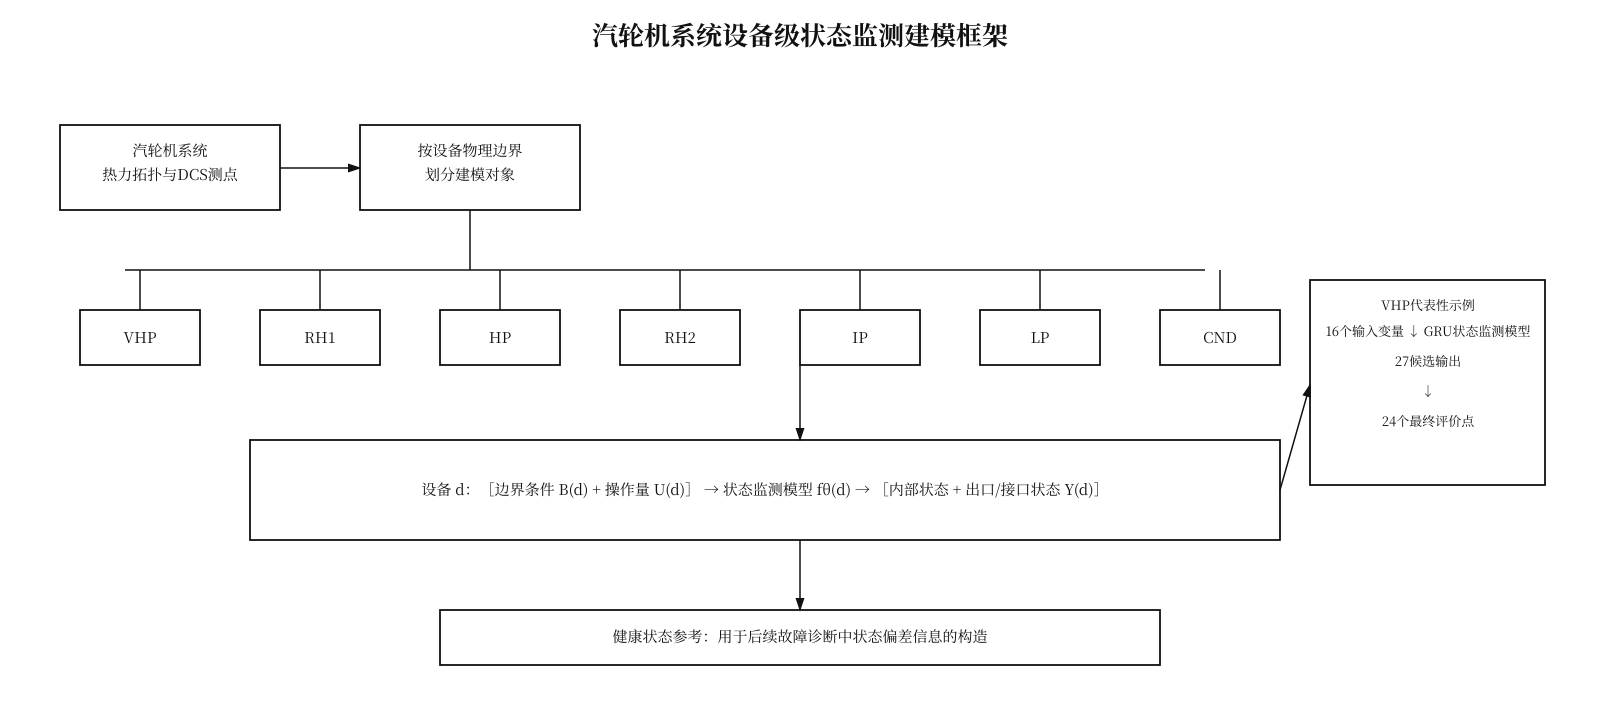
\includegraphics[width=0.94\textwidth]{figures/ch2/fig2_2_device_model_framework_final.svg}
    \caption{汽轮机系统设备级状态监测建模框架}
    \label{fig:device_model_framework_v3}
\end{figure}

\subsubsection{时序数据样本构建}

对于任一设备模型，首先按照统一时间戳对输入与输出测点进行对齐，剔除缺失、重复或时间间隔异常数据。时序模型以连续$L$个采样点构造一个输入窗口，只有窗口内相邻时间戳均保持正常采样间隔时才保留该样本。该处理能够避免因DCS缺测或数据拼接造成不真实的时间跳跃。

输入和输出标准化参数均仅根据训练数据确定。模型选择时，在训练月份内部按照时间顺序划分拟合数据和验证数据，而不进行随机打乱后重新分割，以降低相邻时间序列同时进入训练与验证造成的数据泄露风险。获得最佳训练轮次后，再使用完整训练月份重新训练最终模型，并在独立月份测试数据上评价模型泛化性能。

\subsubsection{本文GRU状态监测网络}

结合模型精度、参数规模和后续设备级扩展需求，本文采用单层小型GRU作为基础网络。对于VHP代表性算例，输入由24个连续采样点组成，每个时间步包含16个运行变量，因此输入张量为$24\times16$。单层GRU隐藏维数设为32，最后隐藏状态先经过LayerNorm进行特征归一化，再通过Dropout(0.05)降低过拟合风险，最后经线性层映射至27个候选状态输出。真实模型结构为
\begin{equation}
    24\times16
    \rightarrow \mathrm{GRU}(32)
    \rightarrow \mathrm{LayerNorm}
    \rightarrow \mathrm{Dropout}(0.05)
    \rightarrow \mathrm{Linear}(27),
\end{equation}
网络总可训练参数量为5755。

图~\ref{fig:gru_architecture_v3}给出了本文GRU网络结构。图中24个时间步上的GRU模块共享同一组网络参数，最后时刻隐藏状态用于形成当前窗口的多维设备状态输出。需要强调的是，网络输出层实际维度为27；后文用于结果统计及故障诊断的24个状态点是在模型完成预测后依据最终诊断节点规则剔除3个候选温度点得到，因此不能将实际训练结构简化描述为Linear(24)。

\begin{figure}[htbp]
    \centering
    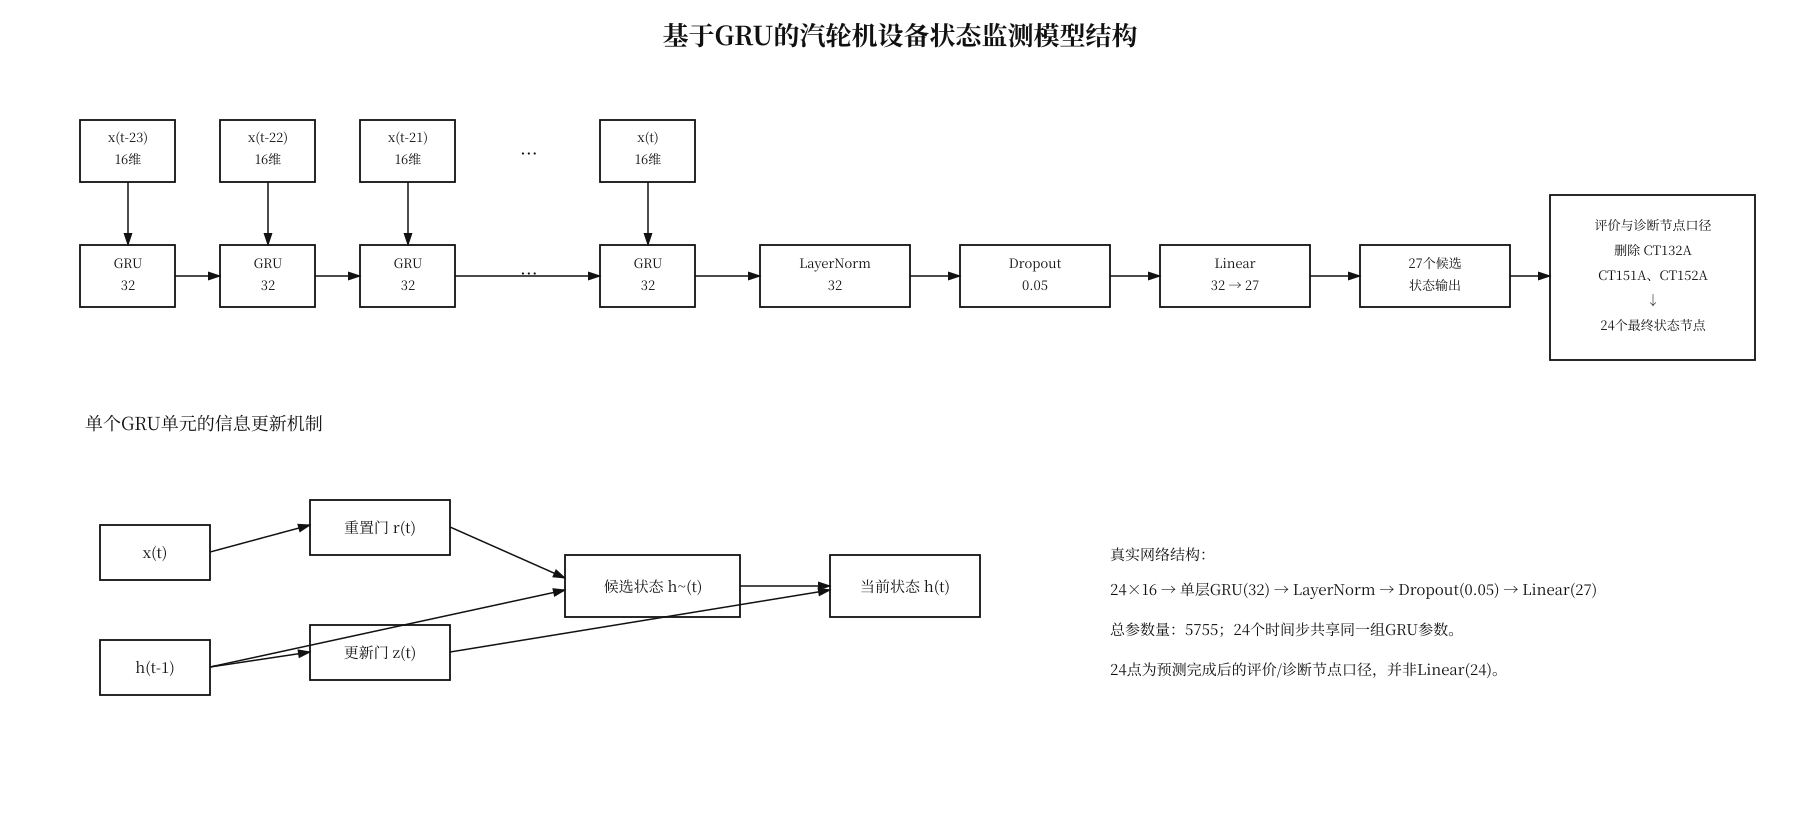
\includegraphics[width=0.98\textwidth]{figures/ch2/fig2_4_gru_architecture_final.svg}
    \caption{基于GRU的汽轮机设备状态监测模型结构}
    \label{fig:gru_architecture_v3}
\end{figure}

\subsubsection{对比模型设置}

为比较不同网络特征提取机制，本文设置ANN、TCN和iTransformer-small作为对比模型。ANN由两层全连接隐藏层构成，不显式引入历史时序信息，主要用于评价静态非线性映射能力；TCN利用因果卷积和不同膨胀系数扩大时间感受野，能够在固定窗口内提取多尺度时序特征\cite{Bai2018TCN}；iTransformer-small采用变量token化和多头注意力机制学习不同变量之间的相关关系\cite{Liu2024iTransformer}。三类网络均与GRU使用相同的原始输入变量和候选输出变量，但ANN不使用24点历史窗口，因此在本文中主要作为无显式时间历史的静态基线，而非完全等价的时序网络对照。

\subsection{工程应用算例}
\label{subsec:vhp_engineering_case_v3}

\subsubsection{研究对象}

为验证上述设备级状态监测方法的工程可行性，本文选取VHP作为代表性对象进行详细分析。VHP位于汽轮机主通流最前端，其入口直接承接锅炉主蒸汽边界，出口连接一次再热系统，同时通过一级抽汽向高压回热系统供汽，因此一个设备即可同时覆盖“入口边界--汽缸内部状态--主排汽--抽汽接口--冷再接口”等多类状态关系，适合用于展示本文建模方法的完整流程。

VHP入口蒸汽由A/B侧主蒸汽管道进入，经调节阀控制后进入汽缸通流级组膨胀做功。主蒸汽压力和温度决定进入汽缸的热力状态，调节阀实际位置体现配汽机构的控制作用，主蒸汽流量及机组有功负荷反映当前整体运行水平。蒸汽在VHP内部膨胀后形成叶片级压力分布和排汽状态，其中部分蒸汽通过一级抽汽支路进入1号高压加热器，其余主流进入冷再系统并送往RH1。因此，VHP状态监测同时涉及本体通流和两个重要外部热力接口。

参照设备过程与测点布置，本文将VHP监测变量按物理作用分为三类输入和四类输出。输入侧包括主蒸汽直接热力边界、调节阀操作量以及机组总体运行条件；输出侧包括VHP本体及主排汽状态、一级抽汽接口、VHP至RH1冷再接口以及缸体与内部蒸汽热状态。与杨昊东高压流化风机算例中分别利用送风参数、阀门反馈、电机负荷和轴承温度表征不同设备状态的处理思路类似，本文不是简单罗列DCS点号，而是根据VHP蒸汽过程解释各类测点在状态监测中的作用。

\subsubsection{输入输出变量及测点配置}

VHP模型最终采用16个输入变量。A/B侧主蒸汽压力和温度各保留3组冗余测点，共12点，用于描述VHP入口热力边界；两侧VHP调节阀实际位置共2点，用于反映本级配汽机构操作状态；机组有功负荷和主蒸汽流量各1点，用于表征整体运行水平和蒸汽通量。上述变量共同构成VHP在常规通流工况下的主要外部作用条件。

输出端实际训练27个候选状态参数。为服务后续故障诊断节点构建，预测完成后删除CT132A、CT151A和CT152A三个候选温度点，最终保留24个状态参数用于本章结果统计。根据物理过程进一步分为四组：Y1为VHP本体及主排汽状态，主要包含叶片级压力、排汽压力及排汽蒸汽温度；Y2为一级抽汽及1号高加接口状态，反映抽汽从VHP向回热系统传递的热力条件；Y3为VHP至RH1的冷再接口状态，用于描述主通流由VHP排汽进入一次再热系统时的状态；Y4为缸体与内部蒸汽状态，主要包括内外缸壁温和内部蒸汽温度等热惯性较强的变量。

不同输出组具有不同状态监测意义。Y1直接反映VHP通流和排汽过程，是判断设备主体状态的主要信息；Y2与抽汽压力和温度相关，可用于反映VHP通流状态变化对回热支路的影响；Y3位于VHP与RH1之间，是后续故障传播和设备接口分析的重要节点；Y4则反映金属结构及内部蒸汽的慢变热状态。四类参数共同覆盖VHP从入口边界到本体、抽汽及下游接口的主要可观测过程。

\subsubsection{数据集及预处理}

本文采用2024年5月正常运行数据训练VHP状态监测模型，2024年6月作为独立测试月份。原始DCS数据采样周期为1~min，经运行状态和数据质量筛选后，训练月份包含43911条有效记录，测试月份包含42710条有效记录；训练负荷范围为280.986--1029.905~MW，测试负荷范围为285.910--1009.141~MW，覆盖了机组较宽的正常运行负荷区间。

对于GRU、TCN和iTransformer-small，将连续24个采样点构成一个时序样本。只有窗口内相邻时间戳均保持1~min间隔时才保留样本，完成窗口构造后GRU训练集包含43759个序列样本，测试集包含42595个序列样本。模型输入和输出均进行StandardScaler标准化，所有均值和标准差仅由训练数据确定。

本章健康模型针对常规通流模式建立，因此当前主模型未将高压旁路动作工况作为输入变量和训练模式。该处理使模型首先针对运行边界相对统一、样本规模充足的正常工况建立稳定健康参考，避免不同运行模式混合对基础模型评价产生额外干扰。

\subsubsection{实验设置及评价指标}

GRU输入序列长度为24，输入维数为16，隐藏单元数为32，采用单层GRU、LayerNorm、Dropout(0.05)和27维线性输出层。训练使用AdamW优化器，初始学习率$1\times10^{-3}$，权重衰减$1\times10^{-4}$，batch size为4096，并将梯度范数裁剪至5.0。训练月份内部按照时间顺序划分模型拟合数据和验证数据，使用ReduceLROnPlateau根据验证损失调整学习率；验证集最优轮次确定后，再在完整训练月份上按相同轮次重新训练最终模型。

模型采用决定系数$R^2$、均方根误差RMSE和平均绝对误差MAE评价：
\begin{equation}
R^2=1-\frac{\sum_{i=1}^{n}(y_i-\hat y_i)^2}{\sum_{i=1}^{n}(y_i-\bar y)^2},
\end{equation}
\begin{equation}
\mathrm{RMSE}=\sqrt{\frac{1}{n}\sum_{i=1}^{n}(y_i-\hat y_i)^2},
\end{equation}
\begin{equation}
\mathrm{MAE}=\frac{1}{n}\sum_{i=1}^{n}|y_i-\hat y_i|.
\end{equation}
其中$y_i$和$\hat y_i$分别表示实际值和模型预测值，$\bar y$为实际样本平均值。由于输出同时包含压力和温度等不同物理量，RMSE和MAE只进行逐测点或相同量纲比较，整体模型性能采用无量纲的24点宏平均$R^2$评价。

\subsubsection{模型训练过程}

模型选择阶段的训练损失和验证损失总体随训练轮次下降，并在后期逐渐稳定。最低验证MSE为0.057533，出现在epoch 161，对应训练MSE为0.043519。根据该结果，将161轮确定为最终训练轮次，随后使用完整2024年5月训练数据重新训练模型，第161轮完整训练集MSE为0.039283。训练和验证损失变化趋势一致，说明当前小型GRU在VHP多输出任务上能够稳定收敛。

需要强调的是，训练损失仅用于模型选择，不能作为判断健康状态模型有效性的唯一依据。本文最终仍采用完全独立的2024年6月运行数据评价模型泛化性能，从而检验模型能否在跨月份运行边界变化情况下继续给出可靠状态参考。

\subsubsection{状态监测结果及模型对比}

在最终24个状态参数上，ANN、TCN、iTransformer-small和GRU-RNN的测试宏平均$R^2$分别为0.9087、0.9397、0.9356和0.9511。GRU取得最高总体精度，相比ANN提高0.0424，相比TCN和iTransformer-small分别提高0.0114和0.0155。逐测点比较中，GRU在24个状态点中的17个点获得四种模型最高$R^2$，说明总体优势并非由少数高精度测点偶然造成。

不同物理状态组的预测难度存在明显差异。GRU在Y1 VHP本体及主排汽状态、Y2一级抽汽接口和Y3 VHP至RH1接口上的平均$R^2$分别达到0.9581、0.9634和0.9569，而Y4缸体与内部蒸汽状态平均$R^2$为0.8893。前三组以压力、主流蒸汽温度和接口状态为主，其变化与主蒸汽边界、阀门动作和负荷较直接相关；Y4包含金属壁温和内部热状态，受热蓄积和历史负荷轨迹影响更明显，因此建模难度更高。

以典型测点进一步分析，超高压缸叶片级压力\#1的GRU测试$R^2$达到0.9979，RMSE为0.1417~MPa，MAE为0.1046~MPa，表明输入边界能够较充分描述该压力状态。对于具有更明显热惯性的排汽温度，模型差异明显增大：超高压排汽蒸汽温度\#1的ANN、TCN、iTransformer-small和GRU测试$R^2$分别为0.8092、0.8492、0.8488和0.8676；排汽蒸汽温度\#3对应值分别为0.8840、0.9153、0.9135和0.9387，时序模型整体优于静态ANN，GRU表现最优。

一级抽汽逆止门后水平管管顶温度的GRU测试$R^2$为0.9529，也高于ANN、TCN和iTransformer-small，说明设备级模型不仅能够描述VHP本体状态，还能够为VHP向高压回热系统传递的抽汽接口建立正常参考。另一方面，超高压内缸壁温90\%处\#1的GRU测试$R^2$仅为0.7346，iTransformer-small为0.7483，明显低于压力和蒸汽温度状态。该结果表明金属温度具有更强长期热惯性，当前24点时间窗口和边界变量仍不能完全解释其变化。本文保留该困难状态，不通过删除低精度测点夸大模型整体性能。

综合四类模型结果，ANN能够学习运行边界与状态之间的基本非线性关系，但对具有动态滞后的热状态表征能力有限；TCN通过因果卷积获得了较好的时序预测性能；iTransformer-small在部分高精度压力状态上表现突出，但当前小模型设置下总体平均精度略低于GRU。GRU在5755个参数的紧凑结构下取得最高24点宏平均$R^2$，并在多数温度和接口状态上保持较稳定性能。因此，本文选取GRU作为汽轮机设备级状态监测的基础模型。其输出将在后续KG-GCN故障诊断章节中作为设备健康状态参考，与实际运行参数共同构成故障诊断所需的动态状态信息。

\subsection{本章小结}

本章针对燃煤机组汽轮机系统故障诊断前的健康状态表征需求，研究了基于GRU的设备级状态监测方法。首先从汽轮机本体主通流、再热、抽汽回热、给水和凝汽器冷端等热力过程出发，分析了不同系统设备之间的介质和能量联系，并将状态监测变量划分为直接热力边界、操作量、设备本体状态、热力接口状态和慢变热状态等不同物理角色。在此基础上提出按照设备物理边界分别建模的统一方法，将直接边界和操作量作为输入，将设备内部、出口及关键接口状态作为输出。

随后系统介绍了RNN的时序建模思想和GRU的门控机制，并进一步给出多变量时间窗口、多输出映射、数据标准化、MSE损失函数以及BPTT参数优化过程。本文采用的实际GRU网络结构为$24\times16\rightarrow$GRU(32)$\rightarrow$LayerNorm$\rightarrow$Dropout(0.05)$\rightarrow$Linear(27)，总参数量5755。

最后以VHP为代表性对象开展工程应用验证。2024年5月训练、2024年6月独立测试结果表明，GRU在最终24个状态参数上的宏平均$R^2$达到0.9511，整体优于ANN、TCN和iTransformer-small，并在24个状态点中的17个点取得最高$R^2$。VHP本体、一级抽汽和冷再接口均获得较高监测精度，证明所建GRU模型能够为汽轮机设备提供较稳定的正常状态参考，为后续基于知识图谱和图卷积网络的故障诊断奠定模型与数据基础。